\frame{
\begin{exampleblock}{Sistema MOLDEAS}
Rendimiento de Consultas en SPARQL.
\end{exampleblock}
}


\frame{
  \frametitle{Rendimiento de Consultas en SPARQL}

\begin{exampleblock}{Objetivo General}<1->
Mejorar el rendimiento de las consultas en SPARQL.
\end{exampleblock}


\begin{block}{1-Definición de los objetivos del experimento}<2->
\begin{enumerate}
 \item ¿Cuáles son las mejoras que se pueden aplicar sobre una consulta en SPARQL para mejorar el tiempo de ejecución?
 \item ¿Cuál es la combinación de mejoras que obtiene un mejor tiempo de respuesta?
 \item ¿Cuál es el coste de la combinación de estas mejoras? 
 \item ¿Existe algún elemento externo de configuración que implique un incremento en el tiempo de ejecución de las consultas? 
 \item ¿Cómo afectan los resultados en la implementación actual del sistema MOLDEAS?
\end{enumerate}

\end{block}

}
% 

\frame{
  \frametitle{Rendimiento de Consultas en SPARQL}

\begin{block}{2-Selección de una regla de asignación de las unidades experimentales a las condiciones de estudio}
\begin{enumerate}
\item Unidad experimental de este estudio será un repositorio RDF.
\item Base documental $\mathcal{D}$ constituida por $1$ millón de anuncios de licitación.
\item Vocabulario controlado, $\mathcal{V}$, del CPV 2008, formado por 10357 códigos/términos distintos.
\item Cada documento $d \in \mathcal{D}$, etiquetado con al menos un código $v \in \mathcal{V}$ y un códigos NUTS.
\item Casos de test $T_k$ (tratamiento) para cada consulta $Q_k$ con características $F_k$.
\item Ejecución de 3 réplicas por cada $T_k$ con reinicio y calentamiento del entorno de pruebas.
\end{enumerate}
\end{block}

}


 \frame{
  \frametitle{Rendimiento de Consultas en SPARQL}
 
 \begin{block}{3-Especificación de las medidas de trabajo en cuanto a la respuesta}<1->
 Tiempo de ejecución en segundos.
\end{block}

\begin{exampleblock}{5-Ejecución de un experimento piloto}<2->
\begin{itemize}
 \item Una muestra de consultas, sólo un año de anuncios de licitación. 
  \item Ejecución de todos los tratamientos.
 \item Toma de tiempos y obtención de resultados.
\end{itemize}
\end{exampleblock}

}

 \frame{
  \frametitle{Rendimiento de Consultas en SPARQL}
 
 \begin{block}{6-Esquematización de los pasos a seguir}<1->
\begin{enumerate}
 \item Preparación y entrenamiento del entorno de ejecución.
 \item Ejecución del script de consultas.
 \item Procesamiento de los resultados.
\end{enumerate}

\end{block}

 \begin{alertblock}{Otros}<2->
\begin{enumerate}
  \item 5-Especificación de un modelo (N/A).
  \item 7-Determinación del tamaño muestral (ya indicado en el punto 1).
  \item 8-Revisión de las decisiones anteriores.
\end{enumerate}

\end{alertblock}

}


\frame{
  \frametitle{Rendimiento de Consultas en SPARQL}
\small
\begin{table}[!ht]
\renewcommand{\arraystretch}{1.3}
\begin{center}
\begin{tabular}{|l|p{2.5cm}|p{3.5cm}|p{2.5cm}|}
\hline
  \textbf{ID} & \textbf{Código CPV inicial} & \textbf{Códigos CPV expandidos} & \textbf{Códigos NUTS}  \\ \hline
  $Q_1$ & 15331137 & 48611000, 48611000, 50531510, 15871210 & UK, PL, RO \\ \hline
  $Q_2$ & 50531510 & 34144100, 44212211, 44212212, 50531500 & ES, FR, DE \\ \hline
  $Q_3$ & 34144100 & 44212211, 31140000, 31140000, 34144100 & PL, CZ, RO \\ \hline
  $Q_4$ & 64122000 & 64216120, 79571000, 15871210, 64121000 & BE, SE, DE \\ \hline
  \hline
  \end{tabular}
  \end{center}
\end{table} 
}


\frame{
  \frametitle{Rendimiento de Consultas en SPARQL}
\small
\begin{table}[!ht]
\renewcommand{\arraystretch}{1.3}
\begin{center}
\begin{tabular}{|l|p{2.5cm}|p{3.5cm}|p{2.5cm}|}
\hline
  \textbf{ID} & \textbf{Código CPV inicial} & \textbf{Códigos CPV expandidos} & \textbf{Códigos NUTS}  \\ \hline
  $Q_5$ & 79320000 & 75241000, 75100000, 75000000, 60112000 & UK, FR, AT \\ \hline
  $Q_6$ & 44100000 & 44110000, 44170000, 44190000, UB03 & NL, SE, DE \\ \hline
  $Q_7$ & 31000000 & 33141000, 39000000, 44000000, 31600000 & DE, IT, HU \\ \hline
  $Q_8$ & 50000000 & 50512000, 50333100, 50530000, 50532300 & UK, IR, FR \\ \hline
  $Q_9$ & 15841400 & 15841300, 15511700, 44921210, 03131400 & ES, FR, DK \\ \hline
  \hline
  \end{tabular}
  \end{center}
\end{table} 
}

\frame{
  \frametitle{Rendimiento de Consultas en SPARQL}
\small
\begin{longtable}[c]{|l|p{8.5cm}|} 
\hline
\textbf{ID} &  \textbf{Descripción}  \\\hline
\endhead
$F_1$ & Consulta simple: $1$ código CPV y $1$ código NUTS \\ \hline
$F_2$ & $F_1$ con uso de la cláusula \texttt{LIMIT} de SPARQL \\ \hline
$F_3$ & Consulta expandida: $n$ códigos CPV y $n$ código NUTS  \\ \hline
$F_4$ & Reescritura de las consultas SPARQL: \texttt{FILTER}, etc.  \\ \hline
$F_5$ & Uso de grafos nombrados en la consulta SPARQL: claúsula \texttt{FROM} \\ \hline
$F_6$ & Separación de las consultas en SPARQL en simples ($F_1$) \\ \hline
$F_7$ & Consultas simples distribuidas con $5$ hilos (1 por código CPV) \\ \hline
\hline
\end{longtable}
}

\frame{
  \frametitle{Rendimiento de Consultas en SPARQL}
\small
\begin{table}[!htb]
\renewcommand{\arraystretch}{1.3}
\begin{center}
\begin{tabular}{|p{2cm}|c|c|c|c|c|c|c|p{2cm}|}
\hline
  \textbf{Test}/ \textbf{Característica}& \textbf{$F_1$} & \textbf{$F_2$} & \textbf{$F_3$} & \textbf{$F_4$} & \textbf{$F_5$} & \textbf{$F_6$} &  \textbf{$F_7$} & \textbf{Nº consultas SPARQL} \\ \hline
   $T_1$ & $\star$ & & & & & & &$1$\\ \hline 
   $T_2$ & $\star$ & & $\star$ & & & & &$1$\\ \hline 
   $T_3$ &  & $\star$ &  & & & & &$1$\\ \hline 
   $T_4$ &  & $\star$ & $\star$ & & & & &$1$\\ \hline 
   $T_5$ &  & $\star$ & $\star$ & $\star$ & & & &$1$\\ \hline 
   $T^{1}_6$ ($n$ CPVs y $m$ NUTS)&  & $\star$ & $\star$ & $\star$ & $\star$ & $\star$ & &$4$\\ \hline 
   $T^{2}_6$ ($\equiv$)&  & $\star$ & $\star$ & $\star$ & $\star$ & $\star$ & $\star$ &$4$\\ \hline 
   $T^{1}_7$ ($1$ CPV y $m$ NUTS) &  & $\star$ & $\star$ & $\star$ &  & $\star$ &  &$5$ \\ \hline 
   $T^{2}_7$ ($\equiv$) & & $\star$ & $\star$ & $\star$ &  & $\star$ & $\star$ &$5$\\ \hline 
   \hline
  \end{tabular}
  \end{center}
\end{table} 
}

\frame{
  \frametitle{Rendimiento de Consultas en SPARQL}
\small
\begin{table}[!htb]
\renewcommand{\arraystretch}{1.3}
\begin{center}
\begin{tabular}{|p{2cm}|c|c|c|c|c|c|c|p{2cm}|}
\hline
  \textbf{Test}/ \textbf{Característica}& \textbf{$F_1$} & \textbf{$F_2$} & \textbf{$F_3$} & \textbf{$F_4$} & \textbf{$F_5$} & \textbf{$F_6$} &  \textbf{$F_7$} & \textbf{Nº consultas SPARQL} \\ \hline
   $T^{1}_8$ ($\equiv$)& & $\star$ & $\star$ & $\star$ & $\star$ & $\star$ &  &$20$\\ \hline 
   $T^{2}_8$ ($\equiv$) & & $\star$ & $\star$ & $\star$ & $\star$ & $\star$ &  $\star$ &$20$\\ \hline 
   $T^{1}_9$ ($1$ CPV y $1$ NUTS ) & & $\star$ & $\star$ & $\star$ &  & $\star$ & &$15$  \\ \hline 
   $T^{2}_9$ ($\equiv$)& & $\star$ & $\star$ & $\star$ & & $\star$ &  $\star$ &$15$\\ \hline 
   $T^{1}_{10}$ ($\equiv$) & & $\star$ & $\star$ & $\star$ & $\star$ & $\star$ & &$60$  \\ \hline 
   $T^{2}_{10}$ ($\equiv$) & & $\star$ & $\star$ & $\star$ & $\star$ & $\star$ & $\star$ &$60$ \\ \hline 
  \hline
  \end{tabular}
  \end{center}
\end{table} 
}



 \frame{
  \frametitle{Rendimiento de Consultas en SPARQL-Resultados Agregados}
 
\begin{columns}[c] % the "c" option specifies center vertical alignment
\column{.5\textwidth} % column designated by a command
\footnotesize
\begin{table}[!htb]
\renewcommand{\arraystretch}{1.3}
\begin{center}
\begin{tabular}{|l|p{2cm}|p{2cm}|}
\hline
  \textbf{Test}& \textbf{$\bar{X}$ Tiempo (seg.)} & \textbf{$\bar{X}$ Ganancia (\%)} \\ \hline
   $T_1$ & $3.21$  & N/A\\ \hline 
   $T_2$ & $3.25$  & $1.21$   \\ \hline 
   $T_3$ & $20.548$ & N/A   \\ \hline 
   $T_4$ & $20.552$ & $-0.02$ \\ \hline 
   $T_5$ & $20.545$ & $-0.01$ \\ \hline 
   $T^{1}_6$ & $20.52$  & $0.14$\\ \hline 
   $T^{2}_6$ & $11.80$ & $74.37$\\ \hline 
    \hline
  \end{tabular}
  \end{center}
\end{table} 


\column{.5\textwidth}
\footnotesize
\begin{table}[!htb]
\renewcommand{\arraystretch}{1.3}
\begin{center}
\begin{tabular}{|l|p{2cm}|p{2cm}|}
\hline
  \textbf{Test}& \textbf{$\bar{X}$ Tiempo (seg.)} & \textbf{$\bar{X}$ Ganancia (\%)} \\ \hline
   $T^{1}_7$ & $15.81$ & $30.58$ \\ \hline 
   \textbf{$T^{2}_7$} & \textbf{$10.51$} & \textbf{$96.54$} \\ \hline
    $T^{1}_8$ & $32.33$ & $-36.11$ \\ \hline 
   $T^{2}_8$ & $18.45$ & $11.21$ \\ \hline 
   $T^{1}_9$ & $22.53$ & $-8.77$ \\ \hline 
   $T^{2}_9$ & $12.61$ & $63.36$ \\ \hline 
   \textbf{$T^{1}_{10}$} & \textbf{$71.01$} & $-70.97$ \\ \hline 
   $T^{2}_{10}$ & $35.08$ & $-40.42$ \\ \hline 
  \hline
  \end{tabular}
  \end{center}
\end{table} 

\end{columns}
}


\frame{
  \frametitle{Rendimiento de Consultas en SPARQL-Resultados Gráficos}

\begin{figure}[!htb]
\centering
	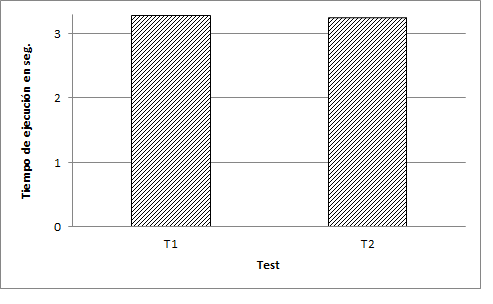
\includegraphics[width=6cm]{./imgs/t1-t2-tiempo}
\caption{Tiempo de ejecución medio con referencia $T_1$.}
\end{figure}
}


\frame{
  \frametitle{Rendimiento de Consultas en SPARQL-Resultados Gráficos}

\begin{figure}[!htb]
\centering
	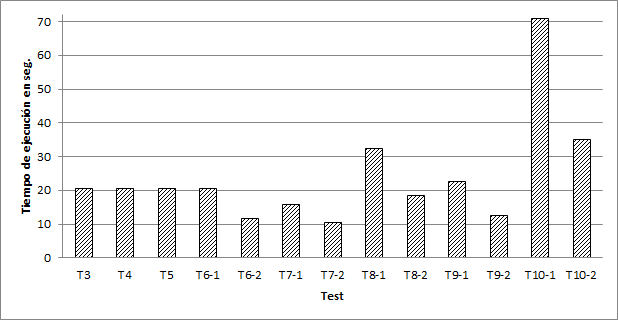
\includegraphics[width=8cm]{./imgs/t3-t10-tiempo}
\caption{Tiempo de ejecución medio con referencia $T_3$.}
\end{figure}
}



\frame{
  \frametitle{Rendimiento de Consultas en SPARQL-Resultados Gráficos}

\begin{figure}[!htb]
\centering
	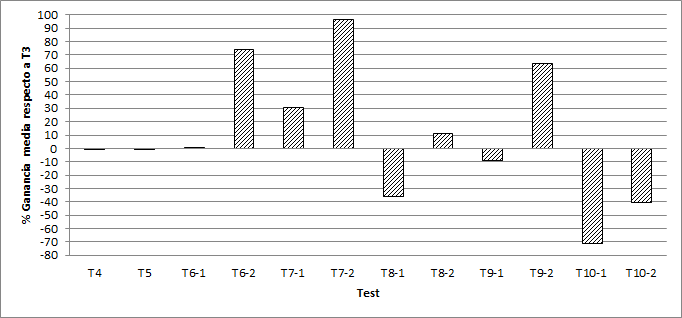
\includegraphics[width=8cm]{./imgs/t3-t10-ganancia}
\caption{Ganancia media con referencia $T_3$ en (\%).}
\end{figure}
}




\frame{
  \frametitle{Rendimiento de Consultas en SPARQL-Resultados}

\begin{block}{Valoración}
 \begin{enumerate}
\item Existen diversas mejoras aplicables a las consultas en SPARQL (LIMIT, FILTER, etc.) que mejoran el rendimiento.
\item El tratamiento $T^{2}_7$ genera el mejor tiempo de ejecución utilizando consultas simples paralelas, con uso de claúsulas LIMIT y FILTER en SPARQL. 
\item La generación de consultas a partir de una expandida no genera sobrecarga significativa en el tiempo de ejecución.
\item Una caché de consultas con resultados predefinidos o índices en el repositorio puede mejorar el rendimiento.
\item Los resultados han implicado una refactorización del código inicial de \texttt{moldeas-api}.
 \end{enumerate}
\end{block}
}
% 
% 
\frame{
  \frametitle{Rendimiento de Consultas en SPARQL-Conclusiones}

\begin{exampleblock}{Puntos Clave}
\begin{itemize}
 \item La \textbf{ejecución} de consultas sobre \textbf{grandes conjuntos de datos} puede ser \textbf{lenta}.
 \item La \textbf{ejecución} de consultas en \textbf{paralelo} \textbf{mejora} el \textbf{tiempo} de ejecución.
 \item El tiempo de generación de las consultas es despreciable.
 \end{itemize}
\end{exampleblock}
}

